\documentclass[conference]{IEEEtran}
\IEEEoverridecommandlockouts
% The preceding line is only needed to identify funding in the first footnote. If that is unneeded, please comment it out.
%Template version as of 6/27/2024

\usepackage{cite}
\usepackage{amsmath,amssymb,amsfonts}
\usepackage{algorithmic}
\usepackage{graphicx}
\usepackage{textcomp}
\usepackage{xcolor}
\usepackage[utf8]{inputenc}
\usepackage[T5]{fontenc}
\usepackage{listings}
\usepackage{url}

% Configure listings package
\lstset{
  basicstyle=\ttfamily\small,
  frame=tb,
  breaklines=true,
  postbreak=\mbox{\textcolor{red}{$\hookrightarrow$}\space},
  literate={_}{{\textunderscore}}1
}

\def\BibTeX{{\rm B\kern-.05em{\sc i\kern-.025em b}\kern-.08em
    T\kern-.1667em\lower.7ex\hbox{E}\kern-.125emX}}
\begin{document}

\title{Xây Dựng Hệ Thống Phân Tán Quản Lý Sinh Viên Theo Hệ Tín Chỉ\\
{\footnotesize \textsuperscript{*}Sử dụng Microservices, Citus, Debezium và Kafka}
\thanks{Nghiên cứu được thực hiện trong khuôn khổ dự án phát triển hệ thống thông tin thế hệ mới.}
}

\author{\IEEEauthorblockN{Nguyễn Ngọc Phú, Vũ Đình Khoa}
\IEEEauthorblockA{\textit{Học viện Công nghệ Bưu chính Viễn thông tại Hồ Chí Minh} \\
\textit{Khoa Công nghệ Thông tin 02}\\
Hồ Chí Minh, Việt Nam \\
Email: \texttt{n22dccn159@student.ptithcm.edu.vn, n22dccn142@student.ptithcm.edu.vn}}
}

\maketitle

\begin{abstract}
Các hệ thống quản lý sinh viên (SMS) truyền thống đang phải đối mặt với áp lực lớn về khả năng mở rộng và tích hợp trong bối cảnh chuyển đổi số. Bài báo này trình bày một kiến trúc phân tán, hướng sự kiện toàn diện để giải quyết các thách thức trên. Giải pháp của chúng tôi kết hợp kiến trúc Microservices cho logic nghiệp vụ, cụm Citus Distributed PostgreSQL cho việc mở rộng cơ sở dữ liệu học vụ, và một CSDL PostgreSQL độc lập cho nghiệp vụ kế toán. Điểm nhấn của kiến trúc là phân mảnh dữ liệu và sử dụng Change Data Capture (CDC) với Debezium và Kafka để đồng bộ dữ liệu một cách bất đồng bộ và tin cậy giữa các thành phần CSDL. Chúng tôi sẽ phân tích sâu về chiến lược sharding, colocation trong Citus và luồng dữ liệu CDC. Kết quả triển khai cho thấy một hệ thống không chỉ có khả năng mở rộng tuyến tính mà còn linh hoạt và dễ bảo trì nhờ sự tách biệt rõ ràng giữa các dịch vụ.
\end{abstract}

\begin{IEEEkeywords}
hệ thống phân tán, microservices, Citus, Debezium, Kafka, Change Data Capture, cơ sở dữ liệu phân tán.
\end{IEEEkeywords}

\section{Giới Thiệu}
Trong môi trường giáo dục đại học ngày càng cạnh tranh, khả năng xử lý và phân tích dữ liệu sinh viên một cách hiệu quả đã trở thành một lợi thế chiến lược. Tuy nhiên, các hệ thống SMS kế thừa, với kiến trúc nguyên khối và CSDL tập trung, thường trở thành nút thắt cổ chai, cản trở việc triển khai các tính năng mới và đáp ứng nhu cầu truy cập ngày càng tăng.

Để phá vỡ những giới hạn này, chúng tôi đề xuất một kiến trúc hiện đại dựa trên các nguyên tắc phân tán và hướng sự kiện. Thay vì một ứng dụng lớn, hệ thống được chia thành các microservices độc lập. Thay vì một CSDL tập trung, chúng tôi sử dụng một kiến trúc CSDL lai: một cụm Citus Distributed PostgreSQL để quản lý dữ liệu học vụ có khối lượng lớn và cần mở rộng, cùng với một CSDL PostgreSQL chuyên biệt cho nghiệp vụ kế toán. Mối liên kết giữa hai hệ thống CSDL này và các microservice khác được xây dựng trên một trục xương sống sự kiện (event backbone) sử dụng Debezium và Kafka, tạo ra một hệ thống linh hoạt, có khả năng chịu lỗi và đồng bộ dữ liệu gần thời gian thực.

\section{Thiết kế cơ sở dữ liệu và đồng bộ hóa}

\subsection{Lược đồ Cơ sở dữ liệu}
Lược đồ cơ sở dữ liệu của hệ thống được cấu thành từ ba loại bảng chính, mỗi loại phục vụ một mục đích riêng biệt nhằm tối ưu hóa hiệu năng và quản lý dữ liệu. Chi tiết về cấu trúc của các bảng này được mô tả trong Bảng \ref{tab:reference_tables}, \ref{tab:distributed_tables}, và \ref{tab:local_tables}.

\begin{table*}[htbp]
\caption{Mô tả các Bảng Tham Chiếu (Reference Tables)}
\label{tab:reference_tables}
\centering
\begin{tabular}{|l|l|l|p{5cm}|}
\hline
\textbf{Tên Bảng} & \textbf{Tên Cột} & \textbf{Kiểu Dữ liệu} & \textbf{Mô tả} \\
\hline
\multicolumn{4}{|c|}{\textbf{\texttt{faculty}}} \\
\hline
\texttt{faculty} & \texttt{faculty\_code} & VARCHAR(10) & Mã khoa (PK) \\
                 & \texttt{faculty\_name} & VARCHAR(50) & Tên khoa \\
\hline
\multicolumn{4}{|c|}{\textbf{\texttt{course}}} \\
\hline
\texttt{course} & \texttt{course\_code} & VARCHAR(10) & Mã môn học (PK) \\
                & \texttt{course\_name} & VARCHAR(50) & Tên môn học \\
                & \texttt{lecture\_credit} & INTEGER & Số tín chỉ lý thuyết \\
                & \texttt{lab\_credit} & INTEGER & Số tín chỉ thực hành \\
\hline
\multicolumn{4}{|c|}{\textbf{\texttt{lecturer}}} \\
\hline
\texttt{lecturer} & \texttt{lecturer\_code} & VARCHAR(10) & Mã giảng viên (PK) \\
                  & \texttt{last\_name} & VARCHAR(50) & Họ giảng viên \\
                  & \texttt{first\_name} & VARCHAR(10) & Tên giảng viên \\
                  & \texttt{faculty\_code} & VARCHAR(10) & Mã khoa (FK) \\
\hline
\multicolumn{4}{|c|}{\textbf{\texttt{global\_class\_code}}} \\
\hline
\texttt{global\_class\_code} & \texttt{class\_code} & VARCHAR(10) & Mã lớp (PK) \\
                            & \texttt{class\_name} & VARCHAR(50) & Tên lớp (PK) \\
\hline
\multicolumn{4}{|c|}{\textbf{\texttt{global\_student\_code}}} \\
\hline
\texttt{global\_student\_code} & \texttt{student\_code} & VARCHAR(10) & Mã sinh viên (PK) \\
\hline
\end{tabular}
\end{table*}

\begin{table*}[htbp]
\caption{Mô tả các Bảng Phân Tán (Distributed Tables) - Cột phân tán: \texttt{faculty\_code}}
\label{tab:distributed_tables}
\centering
\begin{tabular}{|l|l|l|p{5cm}|}
\hline
\textbf{Tên Bảng} & \textbf{Tên Cột} & \textbf{Kiểu Dữ liệu} & \textbf{Mô tả} \\
\hline
\multicolumn{4}{|c|}{\textbf{\texttt{class}}} \\
\hline
\texttt{class} & \texttt{class\_code} & VARCHAR(10) & Mã lớp \\
               & \texttt{class\_name} & VARCHAR(50) & Tên lớp \\
               & \texttt{academic\_year\_code} & VARCHAR(9) & Khóa học \\
               & \texttt{faculty\_code} & VARCHAR(10) & Cột phân phối (PK, FK) \\
\hline
\multicolumn{4}{|c|}{\textbf{\texttt{student}}} \\
\hline
\texttt{student} & \texttt{student\_code} & VARCHAR(10) & Mã sinh viên (PK) \\
                 & \texttt{last\_name} & VARCHAR(50) & Họ sinh viên \\
                 & \texttt{first\_name} & VARCHAR(10) & Tên sinh viên \\
                 & \texttt{class\_code} & VARCHAR(10) & Mã lớp (FK) \\
                 & \texttt{faculty\_code} & VARCHAR(10) & Cột phân phối (PK, FK) \\
\hline
\multicolumn{4}{|c|}{\textbf{\texttt{credit\_class}}} \\
\hline
\texttt{credit\_class} & \texttt{credit\_class\_id} & SERIAL & ID lớp tín chỉ (PK) \\
                      & \texttt{academic\_year} & VARCHAR(9) & Niên khóa \\
                      & \texttt{semester} & INTEGER & Học kỳ \\
                      & \texttt{course\_code} & VARCHAR(10) & Mã môn học (FK) \\
                      & \texttt{faculty\_code} & VARCHAR(10) & Cột phân phối (PK, FK) \\
\hline
\multicolumn{4}{|c|}{\textbf{\texttt{registration}}} \\
\hline
\texttt{registration} & \texttt{credit\_class\_id} & INTEGER & Mã lớp tín chỉ (PK, FK) \\
                      & \texttt{student\_code} & VARCHAR(10) & Mã sinh viên (PK, FK) \\
                      & \texttt{final\_score} & REAL & Điểm cuối kỳ \\
                      & \texttt{faculty\_code} & VARCHAR(10) & Cột phân phối (PK, FK) \\
\hline
\end{tabular}
\end{table*}

\begin{table*}[htbp]
\caption{Mô tả các Bảng Cục bộ trên CSDL Kế toán}
\label{tab:local_tables}
\centering
\begin{tabular}{|l|l|l|p{5cm}|}
\hline
\textbf{Tên Bảng} & \textbf{Tên Cột} & \textbf{Kiểu Dữ liệu} & \textbf{Mô tả} \\
\hline
\multicolumn{4}{|c|}{\textbf{\texttt{student\_basic\_info}}} \\
\hline
\texttt{student\_basic\_info} & \texttt{student\_code} & VARCHAR(10) & Mã sinh viên (PK) \\
                             & \texttt{last\_name} & VARCHAR(50) & Họ sinh viên \\
                             & \texttt{first\_name} & VARCHAR(10) & Tên sinh viên \\
\hline
\multicolumn{4}{|c|}{\textbf{\texttt{tuition}}} \\
\hline
\texttt{tuition} & \texttt{student\_code} & VARCHAR(10) & Mã sinh viên (PK, FK) \\
                 & \texttt{academic\_year} & VARCHAR(9) & Niên khóa (PK) \\
                 & \texttt{semester} & INTEGER & Học kỳ (PK) \\
                 & \texttt{tuition\_fee} & INTEGER & Học phí phải đóng \\
\hline
\multicolumn{4}{|c|}{\textbf{\texttt{tuition\_payment}}} \\
\hline
\texttt{tuition\_payment} & \texttt{student\_code} & VARCHAR(10) & Mã sinh viên (PK, FK) \\
                          & \texttt{academic\_year} & VARCHAR(9) & Niên khóa (PK, FK) \\
                          & \texttt{semester} & INTEGER & Học kỳ (PK, FK) \\
                          & \texttt{payment\_date} & DATE & Ngày đóng tiền (PK) \\
                          & \texttt{amount\_paid} & INTEGER & Số tiền đã đóng \\
\hline
\end{tabular}
\end{table*}

\subsection{Mô Hình Cơ Sở Dữ Liệu Lai}
Chúng tôi chủ đích tách biệt CSDL thành hai hệ thống riêng biệt:
\begin{itemize}
    \item \textbf{Cụm Citus Distributed PostgreSQL:} Chịu trách nhiệm cho tất cả các nghiệp vụ học thuật (quản lý sinh viên, lớp học, điểm số, đăng ký tín chỉ).
    \item \textbf{CSDL PostgreSQL độc lập:} Dành riêng cho phân hệ kế toán, quản lý dữ liệu học phí và các giao dịch tài chính.
\end{itemize}
Mô hình này mang lại nhiều lợi ích. Nó cho phép cụm Citus tập trung hoàn toàn vào việc xử lý các truy vấn phân tích và giao dịch phức tạp của nghiệp vụ học thuật, tận dụng khả năng mở rộng quy mô theo chiều ngang. Trong khi đó, CSDL kế toán được cô lập, tăng cường tính bảo mật cho dữ liệu tài chính và đơn giản hóa việc tuân thủ các quy định về kiểm toán. Sự tách biệt này cũng giúp giảm tải cho hệ thống chính và ngăn ngừa các vấn đề về hiệu năng ở phân hệ này ảnh hưởng đến phân hệ khác.

\subsection{Đồng bộ hóa dữ liệu với Debezium và Kafka}
Để duy trì tính nhất quán dữ liệu giữa hai hệ thống cơ sở dữ liệu, đặc biệt là thông tin cơ bản của sinh viên, chúng tôi đã triển khai một quy trình Thay đổi Dữ liệu (Change Data Capture - CDC) sử dụng Debezium và Apache Kafka. Luồng hoạt động này đảm bảo rằng mọi thay đổi trên bảng \texttt{student} trong cụm Citus sẽ được phản ánh gần như ngay lập tức đến bảng \texttt{student\_basic\_info} trong CSDL kế toán.

\subsubsection{Cấu hình nguồn (Source Configuration) trên Citus}
Quá trình bắt đầu bằng việc cấu hình các worker node của Citus để cho phép CDC. Kịch bản khởi tạo hệ thống (\texttt{start.sh}) thực hiện các bước quan trọng sau:
\begin{itemize}
    \item Kích hoạt tính năng CDC của Citus trên toàn cụm thông qua lệnh: \texttt{ALTER SYSTEM SET citus.enable\_change\_data\_capture = 'on';}
    \item Cấu hình mức độ ghi nhật ký WAL (Write-Ahead Logging) thành \texttt{logical} để cung cấp đủ thông tin cho Debezium: \texttt{ALTER SYSTEM SET wal\_level = 'logical';}
    \item Thiết lập định danh bản sao (replica identity) cho bảng \texttt{student} thành \texttt{FULL}. Điều này đảm bảo rằng các sự kiện \texttt{UPDATE} và \texttt{DELETE} trong WAL sẽ chứa toàn bộ giá trị các cột của hàng bị ảnh hưởng, là điều kiện cần thiết để sink connector hoạt động chính xác.
    \item Tạo một \texttt{PUBLICATION} có tên \texttt{dbz\_student\_shards\_publication} chỉ dành cho bảng \texttt{student}, hoạt động như một kênh phát các sự kiện thay đổi.
\end{itemize}
Do bảng \texttt{student} là một bảng phân tán, nơi các thao tác ghi trong Citus diễn ra trực tiếp trên các worker node, chúng tôi đã triển khai hai Debezium PostgreSQL source connector riêng biệt để đảm bảo không bỏ lỡ bất kỳ sự thay đổi nào trên CSDL, được định nghĩa trong các tệp \texttt{sync\_worker\_0.json} và \texttt{sync\_worker\_1.json}. Mỗi connector được cấu hình để kết nối và lắng nghe các thay đổi từ một worker node tương ứng (\texttt{worker0} và \texttt{worker1}). Cả hai connector cùng theo dõi các thay đổi trên bảng \texttt{public.student} và đẩy các sự kiện thay đổi (tạo, cập nhật, xóa) vào một chủ đề Kafka chung là \texttt{debezium-source.public.student}.

\subsubsection{Cấu hình đích (Sink Configuration) cho CSDL Kế toán}
Ở phía người tiêu thụ, một Debezium JDBC sink connector được triển khai, với cấu hình định nghĩa trong tệp \texttt{target-sink-worker-0.json}. Connector này có nhiệm vụ:
\begin{itemize}
    \item Lắng nghe các thông điệp từ chủ đề Kafka \texttt{debezium-source.public.student}.
    \item Kết nối đến CSDL PostgreSQL của phân hệ kế toán.
    \item Ghi dữ liệu vào bảng \texttt{public.student\_basic\_info}.
\end{itemize}
Cấu hình này sử dụng chế độ ghi là \texttt{upsert}, cho phép connector tự động chèn một bản ghi sinh viên mới hoặc cập nhật một bản ghi đã tồn tại dựa trên khóa chính là \texttt{student\_code}. Hơn nữa, với tùy chọn \texttt{delete.enabled} được đặt thành \texttt{true}, các sự kiện xóa sinh viên từ hệ thống học thuật cũng sẽ được đồng bộ, đảm bảo CSDL kế toán luôn có một bản sao nhất quán và cập nhật của thông tin sinh viên.

\subsection{Lựa chọn cột phân tán và Colocation}
Việc lựa chọn cột phân tán là một quyết định quan trọng trong thiết kế CSDL Citus. Chúng tôi đã chọn \texttt{faculty\_code} (mã khoa) làm cột phân tán cho tất cả các bảng lớn như \texttt{student}, \texttt{class}, \texttt{credit\_class}, và \texttt{registration}.

\section{Thiết kế hệ thống}

\begin{figure}[htbp]
\centering
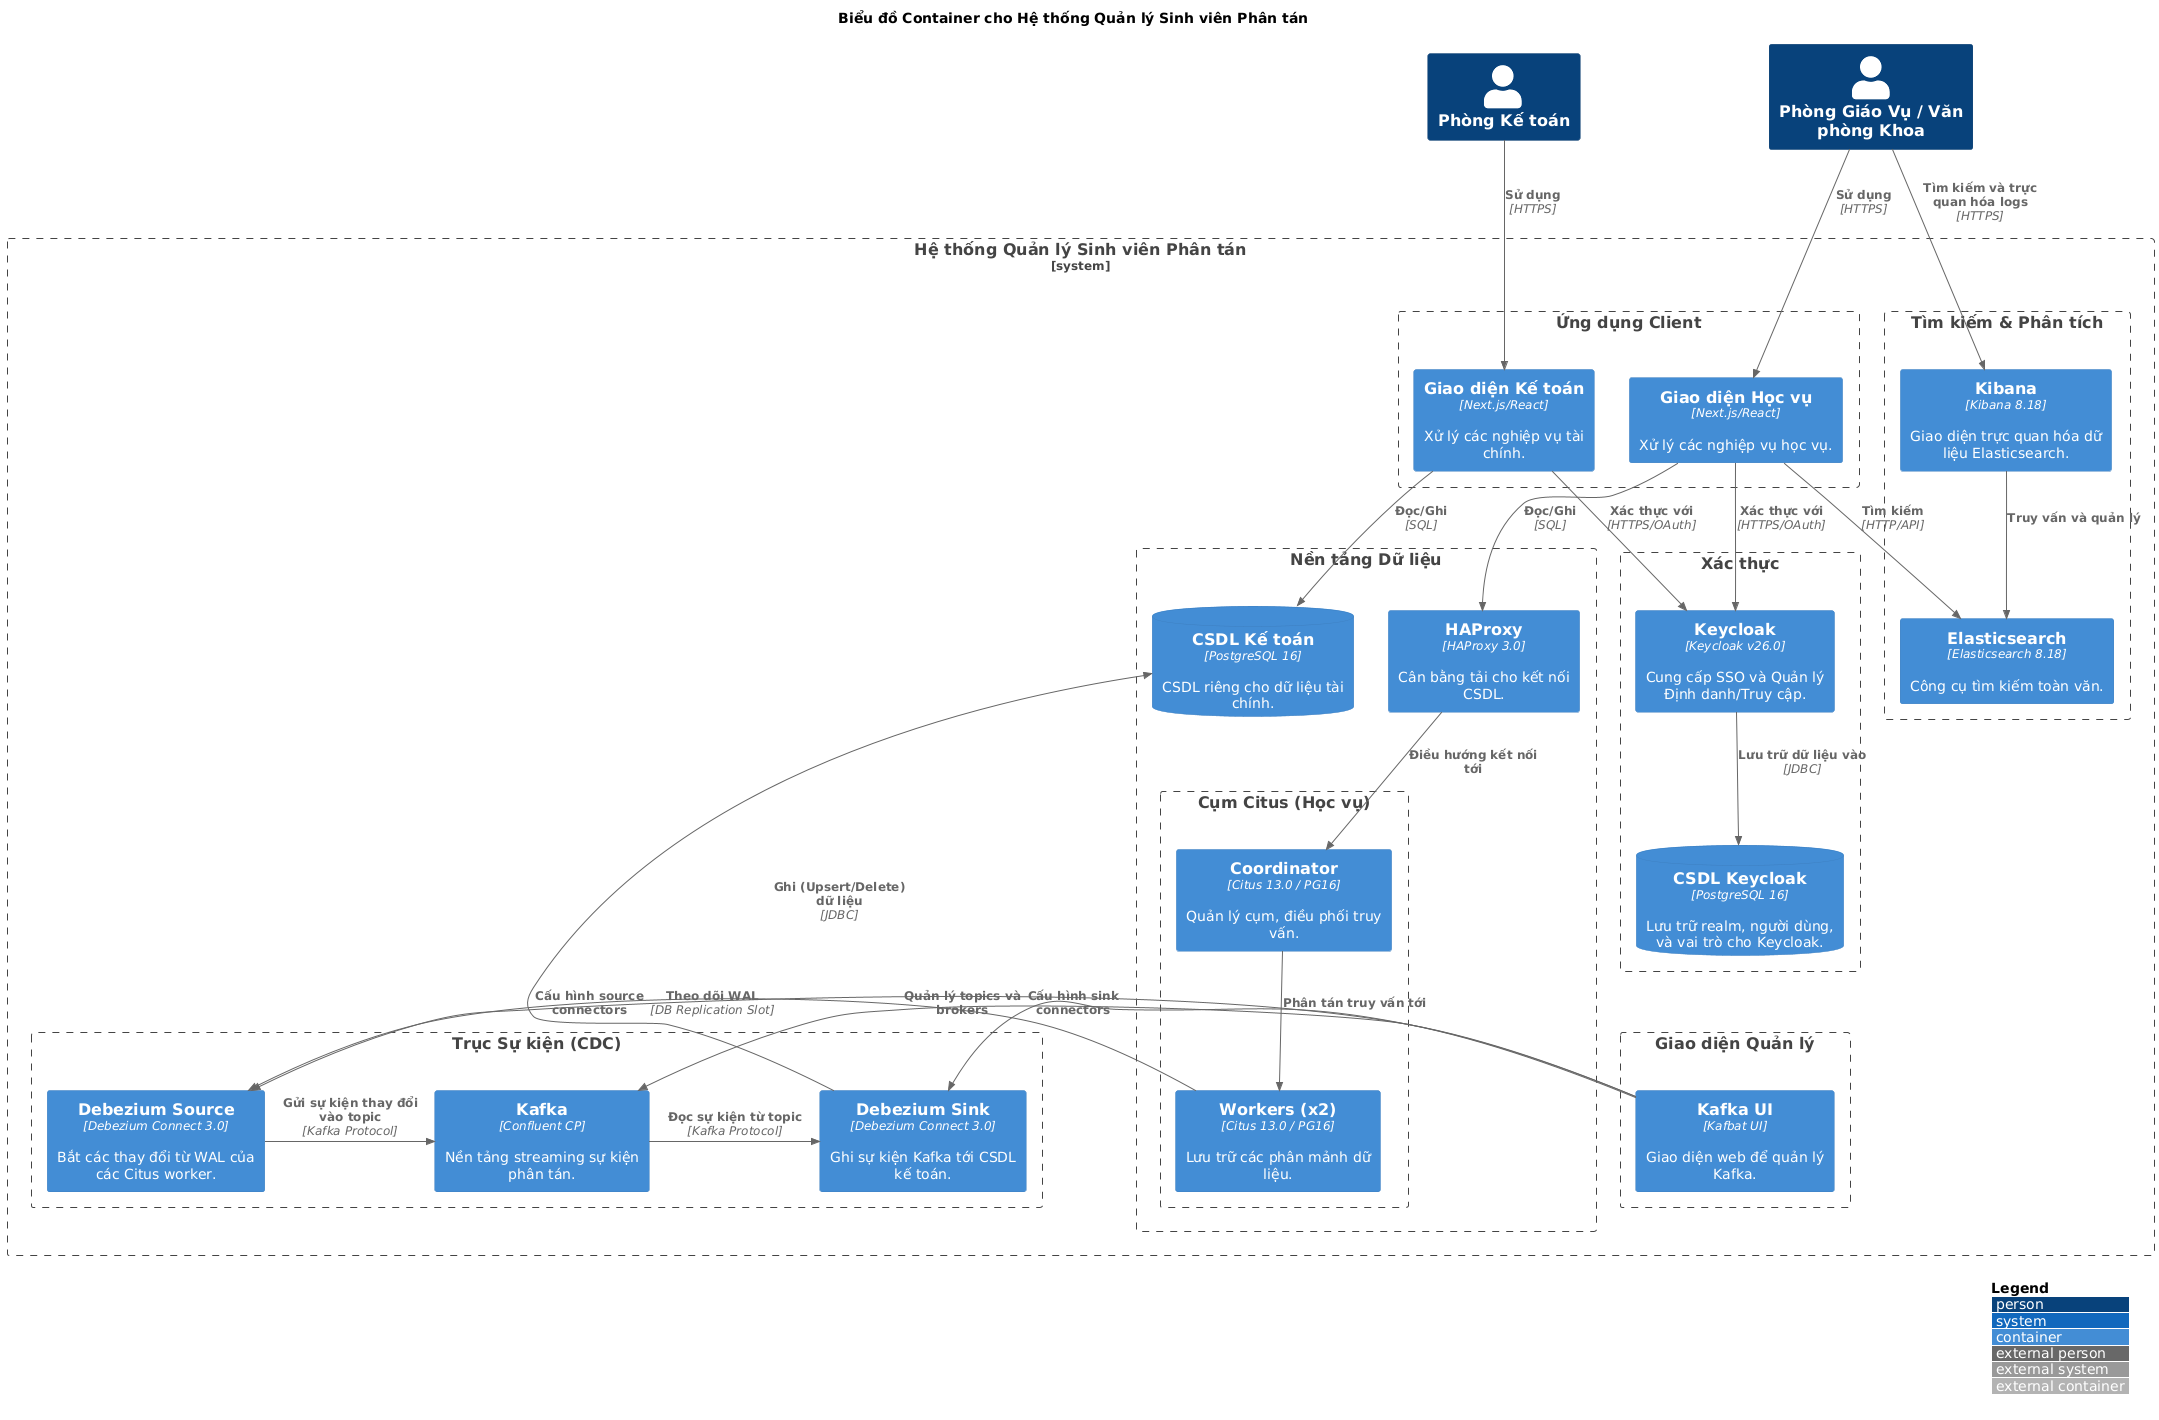
\includegraphics[width=\columnwidth]{C4_Architecture.png}
\caption{Kiến trúc hệ thống theo mô hình C4 (Container).}
\label{fig:c4_diagram}
\end{figure}

Kiến trúc tổng thể của hệ thống (minh họa trong Hình \ref{fig:c4_diagram}) được xây dựng theo mô hình microservices, với môi trường thử nghiệm, chúng tôi triển khai hoàn toàn trên nền tảng container hóa với Docker và được điều phối bởi Docker Compose. Cách tiếp cận này nhằm mô phỏng các dịch vụ có thể được đặt trên các máy chủ khác nhau. Các thành phần chính của hệ thống bao gồm:

\subsection{Các Phân hệ Giao diện Người dùng (Frontend Subsystems)}
Hệ thống cung cấp hai giao diện người dùng độc lập, được xây dựng bằng Next.js, phục vụ cho hai nhóm người dùng riêng biệt:
\begin{itemize}
    \item \textbf{Academic UI}: Giao diện dành cho các nhân viên học vụ (Phòng Giáo Vụ, Văn phòng Khoa) để thực hiện các nghiệp vụ như quản lý khoa, giảng viên, lớp học, sinh viên và điểm số. Giao diện này tương tác trực tiếp với Cụm CSDL Citus thông qua cổng cân bằng tải HAProxy.
    \item \textbf{Accounting UI}: Giao diện dành cho nhân viên phòng kế toán, cho phép quản lý học phí và theo dõi các khoản thanh toán của sinh viên. Giao diện này kết nối trực tiếp đến CSDL kế toán độc lập để đảm bảo tính an toàn và cô lập cho dữ liệu tài chính.
\end{itemize}

\subsection{Dịch vụ Xác thực và Phân quyền (Authentication \& Authorization)}
Toàn bộ việc quản lý danh tính và kiểm soát truy cập trong hệ thống được tập trung hóa bởi \textbf{Keycloak}. Khi người dùng đăng nhập vào một trong hai giao diện, họ sẽ được chuyển hướng đến trang đăng nhập của Keycloak. Sau khi xác thực thành công, Keycloak cấp phát một JSON Web Token (JWT) chứa thông tin người dùng và vai trò của họ (ví dụ: "Phòng Giáo Vụ", "Phòng Kế toán"). Các giao diện người dùng sau đó sẽ đính kèm JWT này vào mỗi yêu cầu API gửi đến backend, và backend sẽ xác thực token này để quyết định người dùng có quyền thực hiện hành động đó hay không. Mô hình này giúp tách biệt logic xác thực ra khỏi các ứng dụng, dễ dàng quản lý người dùng và tăng cường bảo mật.

\subsection{Cổng vào và Cân bằng tải CSDL (Database Gateway \& Load Balancer)}
Để tăng cường tính sẵn sàng cao và đơn giản hóa việc kết nối cho các ứng dụng, chúng tôi sử dụng \textbf{HAProxy} làm cổng vào và cân bằng tải cho CSDL Citus. Mọi kết nối từ Academic UI đến CSDL không trỏ trực tiếp đến Citus coordinator mà sẽ đi qua HAProxy. HAProxy được cấu hình để chuyển tiếp lưu lượng đến coordinator node đang hoạt động. Trong tương lai, nếu hệ thống có nhiều coordinator để dự phòng (failover), HAProxy có thể tự động chuyển hướng kết nối đến coordinator còn lại khi có sự cố, giúp giảm thiểu thời gian gián đoạn dịch vụ.

\subsection{Hệ thống Giám sát và Ghi log (Monitoring \& Logging)}
Với một hệ thống phân tán gồm nhiều thành phần, việc giám sát và quản lý log tập trung là vô cùng quan trọng. Chúng tôi sử dụng bộ đôi \textbf{Elasticsearch và Kibana} cho mục đích này. Mọi dịch vụ trong hệ thống (UI, Keycloak, Debezium) được cấu hình để đẩy log của chúng về Elasticsearch. Elasticsearch đóng vai trò là một công cụ tìm kiếm và phân tích mạnh mẽ, lưu trữ và đánh chỉ mục các log này. \textbf{Kibana} cung cấp một giao diện web trực quan, cho phép các nhà phát triển và quản trị viên hệ thống dễ dàng tìm kiếm, lọc, và trực quan hóa log, giúp nhanh chóng phát hiện và chẩn đoán sự cố trên toàn hệ thống.

\section{Thảo Luận}
\subsection{Ưu điểm của Kiến trúc}
Kiến trúc được đề xuất mang lại nhiều lợi ích đáng kể.
\begin{itemize}
    \item \textbf{Kiến trúc linh hoạt, tách biệt}: Luồng CDC giúp các dịch vụ hoàn toàn độc lập, dễ dàng thay đổi hoặc nâng cấp một dịch vụ mà không ảnh hưởng đến các dịch vụ khác.
    \item \textbf{Đồng bộ tin cậy}: Kafka đảm bảo các sự kiện sẽ được gửi đi (at-least-once semantics), và Debezium đảm bảo không bỏ lỡ thay đổi nào từ CSDL.
    \item \textbf{Hiệu suất truy vấn cao}: Chiến lược sharding và colocation thông minh trong Citus giúp tối ưu hóa phần lớn các truy vấn nghiệp vụ hàng ngày.
    \item \textbf{Khả năng mở rộng toàn diện}: Có thể mở rộng CSDL bằng cách thêm worker node, mở rộng năng lực xử lý sự kiện bằng cách thêm Kafka broker, và mở rộng nghiệp vụ bằng cách thêm microservice.
\end{itemize}

\subsection{Hạn chế}
\begin{itemize}
    \item \textbf{Độ phức tạp vận hành cao}: Quản lý một hệ thống với nhiều thành phần (Citus, Kafka, Debezium, Keycloak) đòi hỏi kiến thức sâu và công cụ giám sát mạnh mẽ.
    \item \textbf{Tính nhất quán sau cùng (Eventual Consistency)}: Dữ liệu giữa CSDL học vụ và kế toán có một độ trễ nhỏ (dù rất thấp). Điều này cần được xem xét trong thiết kế nghiệp vụ.
\end{itemize}

\section{Kết Luận}
Bài báo này đã trình bày một kiến trúc chi tiết và hiện đại cho hệ thống quản lý sinh viên phân tán. Bằng cách sử dụng Citus cho khả năng mở rộng CSDL, và Debezium/Kafka cho việc đồng bộ dữ liệu hướng sự kiện, chúng tôi đã xây dựng được một nền tảng vững chắc, hiệu suất cao và linh hoạt. Mô hình này không chỉ giải quyết các bài toán hiện tại mà còn mở ra nhiều khả năng phát triển trong tương lai, như tích hợp các hệ thống phân tích dữ liệu lớn hoặc các mô hình AI/ML trực tiếp trên luồng sự kiện.

\section*{Lời Cảm Ơn}
Chúng tôi xin chân thành cảm ơn sự đóng góp của cộng đồng mã nguồn mở đã tạo ra các công cụ tuyệt vời như PostgreSQL, Citus, Debezium, Kafka và Keycloak.

\begin{thebibliography}{00}
\bibitem{b1} G. Hohpe and B. Woolf, ``Enterprise Integration Patterns: Designing, Building, and Deploying Messaging Solutions,'' Addison-Wesley, 2003.
\bibitem{b2} Microsoft Corporation, ``Citus Documentation: Distributed PostgreSQL for Multi-Tenant and Real-Time Analytics Workloads,'' 2023.
\bibitem{b3} Debezium Authors, ``Debezium Documentation,'' Red Hat, 2023. [Online]. Available: \url{https://debezium.io/documentation/reference/}
\bibitem{b4} C. Richardson, ``Microservices Patterns: With Examples in Java,'' Manning Publications, 2018.
\bibitem{b5} J. Kreps, N. Narkhede, and J. Rao, ``Kafka: a Distributed Messaging System for Log Processing,'' in Proc. NetDB, 2011.
\bibitem{b6} M. Kleppmann, ``Designing Data-Intensive Applications: The Big Ideas Behind Reliable, Scalable, and Maintainable Systems,'' O'Reilly Media, 2017.
\end{thebibliography}

\end{document}
